%%=============================================================================
%% Methodologie
%%=============================================================================

\chapter{\IfLanguageName{dutch}{Methodologie}{Methodology}}%
\label{ch:methodologie}

Het onderzoek omvat een literatuurstudie (Hoofdstuk 2), waarin technologieën en methoden voor tekstvereenvoudiging voor leerlingen met dyslexie in de derde graad van het middelbaar onderwijs worden beschreven. Hoofdstukken 4 en 5 presenteren een lijst van benodigde functionaliteiten en een stappenplan voor de ontwikkeling van een prototype. In Hoofdstuk 6 wordt een vergelijkende studie uitgevoerd om de meest geschikte tools te bepalen voor het vereenvoudigen van wetenschappelijke artikelen voor leerlingen met dyslexie. Het doel is om te bepalen aan welke criteria een vereenvoudigde tekst moet voldoen om leerlingen met dyslexie in de derde graad van het middelbaar onderwijs te ondersteunen.


\chapter{Requirementsanalyse}

In deze onderzoeksfase worden verschillende tools getest en vergeleken met manuele tekstvereenvoudiging. De vereenvoudigingstechnieken die als gunstig zijn beoordeeld in Hoofdstuk 2, evenals de aspecten waar ontwikkelaars zich bewust van moeten zijn, worden meegenomen in de requirementsanalyse. Deze analyse is verdeeld tussen toepassingen die momenteel in het onderwijs worden gebruikt en online tools die leraren kunnen gebruiken. Gratis beschikbare taalmodellen, zoals GPT-3 of vooraf getrainde taalmodellen zoals BART-SC, worden ook in de analyse opgenomen. Op basis van de capaciteiten en functionaliteiten van de verschillende tools wordt een shortlist opgesteld met de benodigde functionaliteiten om teksten te vereenvoudigen voor middelbare scholieren in de derde graad met dyslexie.

\section{Tekstanalyse}

Geen tool in de shortlist biedt transparantie over keuzes van het taalmodel. Beslissingen zoals CWI worden niet aangegeven door het taalmodel. Geen enkel softwarepakket of hulpmiddel biedt standaard een visuele weergave van waarom een taal- of AI-model een zin als moeilijk of belangrijk beschouwt, of waarom het model een kernwoord heeft gekozen. Dit komt overeen met de bevindingen van \textcite{Gooding2019}. Het GPT3-model en het verwante Bing-model doen dit echter wel wanneer het taalmodel hier expliciet om wordt gevraagd. SciSpace houdt hier geen rekening mee en verwerpt de vraag. Het stellen van vragen aan het taalmodel biedt weliswaar een alternatief, maar het schrijven van efficiënte prompts valt volgens \textcite{} buiten het bereik en de capaciteiten van de gemiddelde eindgebruiker. Deze prompt kan worden aangeboden in de vorm van een intuïtieve knop. Simplish geeft nadien een vergelijkende weergave met de oorspronkelijke tekst en de vereenvoudigde tekst. Met gebruik van kleurcodes worden de verschillende transformaties aangeduid, maar is enkel bij de uitvoer op de site terug te vinden.

\begin{figure}[H]
	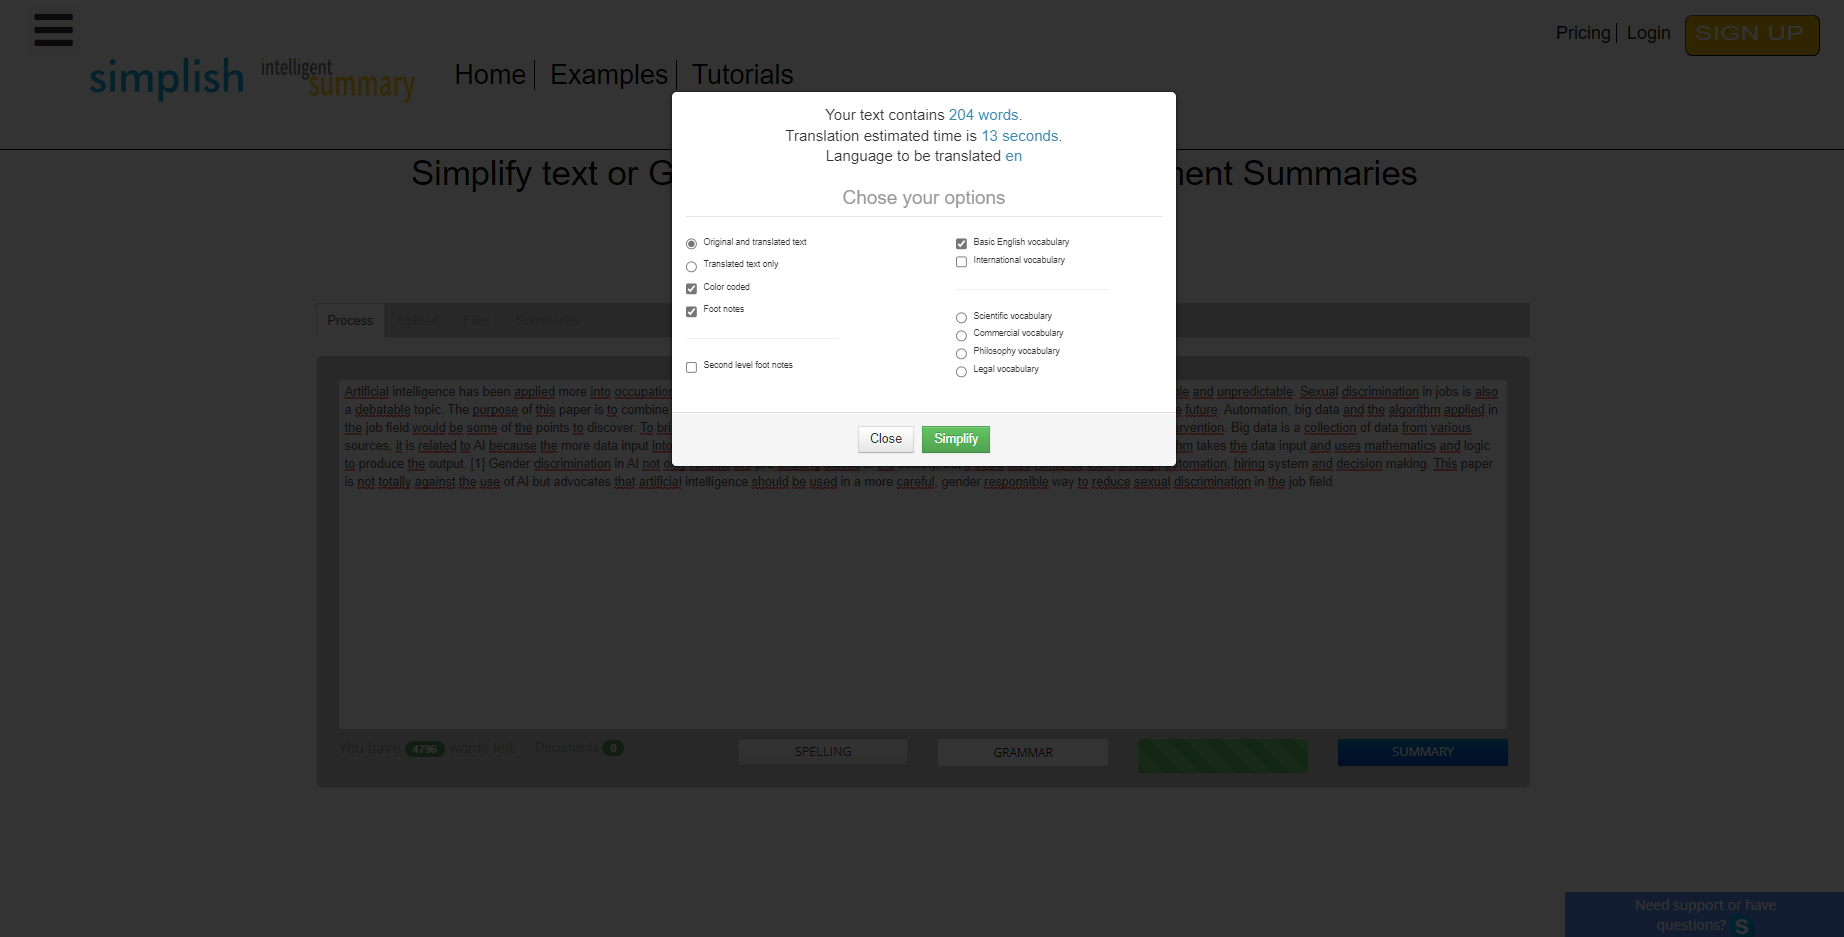
\includegraphics[width=\linewidth]{img/simplish-input.png}
\end{figure}

\begin{figure}[H]
	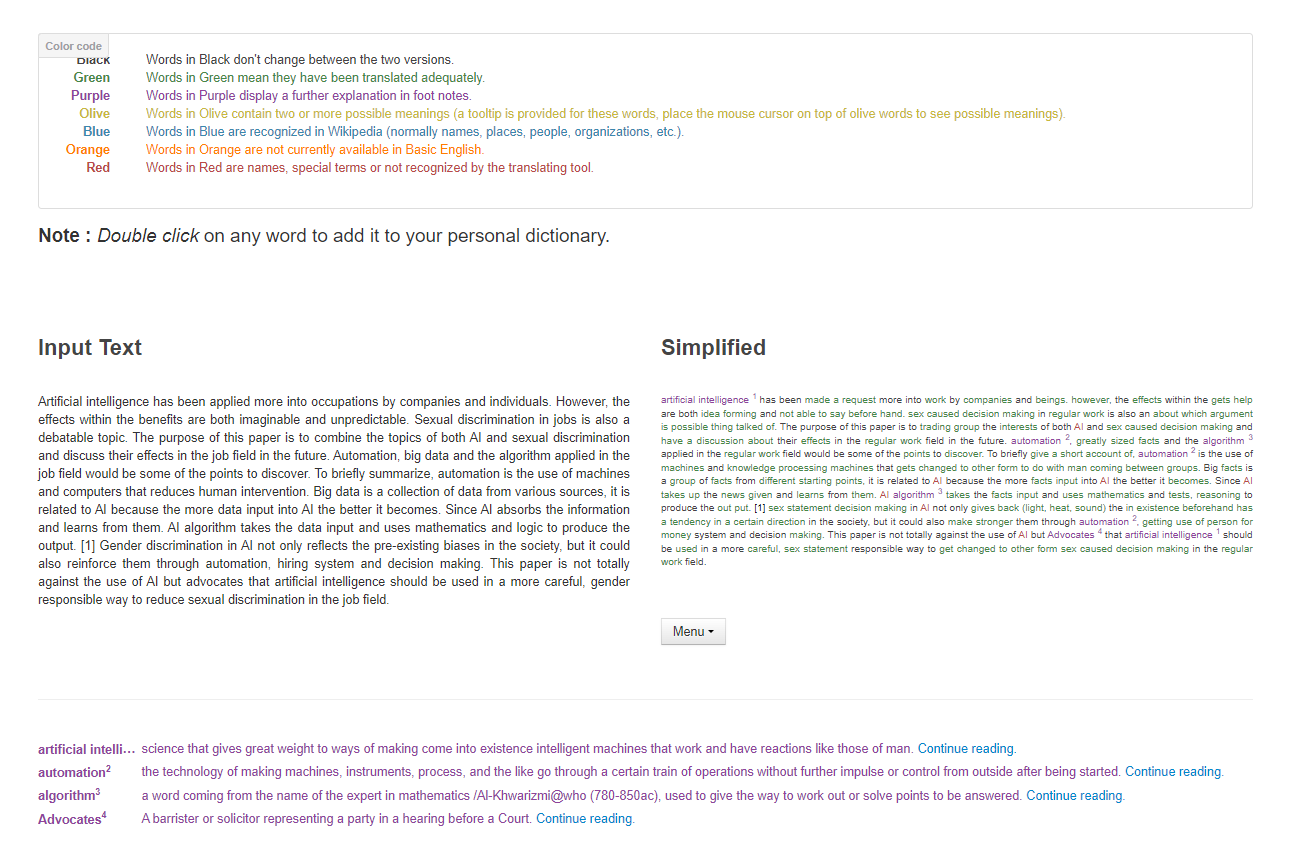
\includegraphics[width=\linewidth]{img/simplish-output.png}
\end{figure}

\section{Lexicale vereenvoudiging}

Momenteel zijn de verschillende softwaretools beschikbaar in het middelbaar onderwijs en Simplish die in staat zijn om woordenlijsten op te maken. Kurzweil biedt daarnaast de mogelijkheid om synoniemen op te vragen voor een bepaald woord, en de gebruiker kan zelf kiezen welk woordenboek gebruikt moet worden voor het opzoeken van definities. Woordenlijsten kunnen alleen automatisch gegenereerd worden met behulp van GPT-taalmodellen door middel van prompts. Het gebruik van GPT-modellen voor het vereenvoudigen van teksten vereist echter wel expliciete aanwijzingen. Deze modellen houden ook rekening met woordambiguïteit en wetenschappelijk of vakjargon. Er zijn echter maar weinig softwarepakketten beschikbaar die rekening houden met ambiguïteit, idiomen en vooraf gedefinieerde achtergrondkennis. Verwante GPT-modellen zijn in staat om zinnen te vereenvoudigen terwijl ze rekening houden met deze drie aspecten. HuggingFace-taalmodellen zoals SC en BART-SC passen moeilijke woorden aan en zijn bestand tegen ambiguïteit en idiomen, maar houden geen rekening met vooraf gedefinieerde woordenschat.

\section{Syntactische vereenvoudiging}

Op dit moment zijn de erkende softwaretools in het middelbaar onderwijs niet in staat om de oorspronkelijke tekst te transformeren, waardoor syntactische vereenvoudiging niet aan de orde is. Online webtoepassingen bieden ook minder functionaliteiten om de moeilijkheidsgraad van zinsyntaxis te verlagen. Het aanpassen van tangconstructies, verwijswoorden, voorzetseluitdrukkingen, samengestelde werkwoorden en onregelmatige werkwoorden is een uitdaging voor deze toepassingen. Het schrijven in de actieve stem kan ook problematisch zijn. Alleen vooraf gedefinieerde prompts maken het mogelijk om deze transformaties uit te voeren. Hoewel de GPT-3 taalmodellen in staat zijn om zinsyntaxtransformaties uit te voeren, kunnen ze soms problemen ondervinden bij het verwerken van alle meegegeven transformaties, en er is geen garantie dat deze modellen alle transformaties met slechts één prompt kunnen uitvoeren. Taalmodellen van HuggingFace houden minder rekening met het aanpassen van de zinsyntaxis en blijft vrijwel identiek.

\section{Samenvatten}

Op dit moment laten erkende tools in het onderwijs gebruikers toe om zinnen te markeren, waarna deze gemarkeerde zinnen aan elkaar worden geplakt. Hierdoor blijft de semantiek van de tekst gelijk, maar kan de resulterende tekst samenhang missen. Parafraseren of abstraherend samenvatten is momenteel niet mogelijk met beschikbare software in het onderwijs. Er zijn echter geavanceerde taalmodellen zoals BERT of GPT-3 die meer functionaliteiten bieden, waaronder abstraherend samenvatten op basis van gemarkeerde zinnen of woorden gekozen door de gebruiker. Experimenten met teksten hebben aangetoond dat GPT en Bing AI de nadruk leggen op het behouden van bronreferenties. Als er expliciet om wordt gevraagd, kan de Bing chatbot bronnen teruggeven die buiten het oorspronkelijke artikel te vinden zijn.

\section{Personalisatie en verdere functionaliteiten}

Vereenvoudigde zinnen of tekstinhoud met OpenAI's Codex of GPT-3 engine kan in een tabel worden gegoten of opsommingen gemaakt worden om zo de tekst overzichtelijker weer te geven. Ontwikkelaars kunnen echter door het aanspreken van deze modellen door de tabel in een structuur zoals Markdown, HTML of LateX op te vragen. Andere taalmodellen -en vereenvoudigingstools houden het bij doorlopende tekst, waarvan sommigen deze uitvoer opsplitsen per paragraaf en sommigen deze als één volledige paragraaf uitprinten. Achtergrondkleur, lettertype- en grootte, marge, regelafstand en spatiëring tussen leestekens aanpassen zijn onbestaand bij eender welke tool in de longlist.

\section{Voor ontwikkelaars}

% In mindere mate zijn er beperkingen voor de tekstsoftware die momenteel in het onderwijs wordt ingezet. Ontwikkelaars kunnen echter geen API aanspreken waarvan de volgende softwarepakketten gebruik maakt, al zijn er wel taalmodellen vrij beschikbaar op HuggingFace die tekstvereenvouding mogelijk maken voor Engelstalige of meertalige teksten. Het uittesten en verkennend onderzoeken was niet mogelijk om het gebruikte taalmodel te achterhalen. Ontwikkelaars moeten rekening houden bij de karakter- of tokenlimiet bij alle modellen of tools. Dit hindert ontwikkelaars bij het ontwerpen en ontwikkelen van software waarbij grote documenten vanaf twee tot drie pagina's voltekst, moeten opgebroken worden in kleinere subdelen. Wetenschappelijke artikelen volgen een logische structuur, dus hier kunnen ontwikkelaars op inspelen. De meeste software is vrij beschikbaar, al zijn niet alle functionaliteiten vrij ter beschikking tot het grote publiek. De GPT-modellen, met uitzondering op chatbots, vereisen het gebruik van een API-sleutel. Het gebruik van deze sleutel is gekoppeld aan \textit{payment subscription} van OpenAI. Alle vermelde modellen maken gebruik van een black-box model. Geen taalmodel is ertoe in staat om duidelijk aan te geven waarom een zin als moeilijk wordt bestempeld, of waarom een woord als moeilijk werd bepaald. Dit sluit aan bij de bevindingen van \textcite{Gooding2022}. \textit{Black-box} taalmodellen zijn dominant aanwezig, maar de zoektocht naar een white-box taalmodel van eenzelfde caliber is niet evident.

Momenteel zijn er beperkingen voor erkende tekstsoftware in het onderwijs, maar er zijn taalmodellen beschikbaar op HuggingFace die tekstvereenvoudiging mogelijk maken voor Engelstalige of meertalige teksten. Het gebruikte taalmodel kan echter niet worden achterhaald en ontwikkelaars moeten rekening houden met de karakter- of tokenlimiet bij alle modellen of tools, wat het ontwerp en de ontwikkeling van software bemoeilijkt bij grote documenten. Hoewel de meeste software vrij beschikbaar is, vereisen GPT-modellen het gebruik van een API-sleutel die gekoppeld is aan een betalingsabonnement van OpenAI. Alle modellen zijn \textit{black-box} modellen en kunnen niet duidelijk aangeven waarom een zin als moeilijk wordt bestempeld of waarom een woord als moeilijk wordt bepaald, wat overeenkomt met de bevindingen van \textcite{Gooding2022}.

\section{Requirements}

% Zinnen of paragrafen vereenvoudigen moet intuïtiever worden aangeboden. Gebruikers moeten zinnen kunnen aanduiden die zij willen vereenvoudigen op basis van meegegeven parameters zoals de lengte of het vermijden van een bepaalde constructie. Het prototype moet personaliseerbaar zijn. Huidige tools ontbreken personalisatie. Weergave zoals lettertypes -en groottes, marges en achtergrondkleur moet personaliseerbaar zijn in de webtool als het uitvoerbestand door de eindgebruiker. Deze parameters moeten in de uitvoer van vereenvoudigde teksten ook aanpasbaar zijn. Het gebruikte taalmodel en indicatie waarom Complex Word Identification mogelijk wordt gemaakt moet benadrukt worden in het prototype. Alsook moet de bron van bijkomende uitleg bij woordenschat vermeld worden. Aanvullend moet het prototype aan de gebruiker kunnen zeggen welke prompt werd meegegeven. Huidige tools ontbreken transparantie. Een prototype voor tekstvereenvoudiging moet op een intuïtieve manier prompts mogelijk maken. Knoppen met vooraf gedefinieerde prompts kunnen het schrijven van prompts vervangen.  De prompt is bij deze modellen de doorslaggevende factor waarbij een bedachtzame voorbereiding moet worden toegediend door de gebruiker. Door deze vereisten te volgen, kan de tool de leesbaarheid van de tekst verbeteren en begrijpelijker maken voor een breder publiek. Aanvullend kan het prototype functies aanbieden die meer inzicht geven over de teksten, zoals de moeilijk leesbare zinnen volgens leesbaarheidsformules.

Een prototype voor tekstvereenvoudiging moet intuïtiever zijn, zodat gebruikers zinnen kunnen aanduiden die ze willen vereenvoudigen op basis van parameters zoals lengte of type constructie. Personalisatie is ook belangrijk, zodat de weergave en parameters kunnen worden aangepast aan de voorkeur van de eindgebruiker. Het taalmodel en de bron van bijkomende uitleg bij woordenschat moeten duidelijk worden aangegeven in het prototype, en er moet transparantie zijn over de gebruikte prompt. De tool moet de leesbaarheid van de tekst verbeteren en begrijpelijker maken voor een breder publiek. Een prototype kan ook functies bevatten die meer inzicht geven in de tekst, zoals de moeilijk leesbare zinnen volgens leesbaarheidsformules. Om het proces te vergemakkelijken, kunnen vooraf gedefinieerde prompts worden aangeboden als knoppen in plaats van dat gebruikers ze zelf moeten schrijven.

\section{Conclusie}

Huidige tools hebben elk een uitblinkende functionaliteit, maar er is geen manusje-van-alles. Daarnaast ontbreken deze personalisatie en transparantie. De uitgeteste toepassingen gebruiken een mix tussen vrij beschikbare modellen en API's en zelfgemaakte taalmodellen die niet aangesproken kunnen worden. Promptgebaseerde toepassingen kunnen veelbelovende vereenvoudigde teksten genereren, maar er moet een intuïtieve manier worden aangeboden aan gebruikers. Zo hoeven zij niet aan prompt engineering te doen. De requirementsanalyse wijst uit dat het prototype een duidelijke opsplitsing moet maken tussen de verwachtte functionaliteiten voor een scholier als voor een docent die een vereenvoudigde tekst wilt laten maken voor een scholier. Scholieren met dyslexie in de derde graad van het middelbaar onderwijs hebben nood aan een ondersteunende tool die hen toelaat om meer info rond zinnen of woorden op te halen, zodat zij de teksten beter kunnen lezen zonder dat de zinnen hun semantiek verliezen of zodat de scholieren niet de nodige kennis ontbreken zoals jargon of zinsstructuren. De docent daarentegen zal een overzicht moeten kunnen krijgen van de oorspronkelijke tekst, alsook keuzes aangereikt moeten krijgen waaraan de vereenvoudigde tekst kan voldoen. De resulterende tekst wordt in PDF of HTML-vorm aan de eindgebruiker aangereikt.

\chapter{Prototype voor tekstvereenvoudiging}

Dit hoofdstuk omschrijft de ontwikkeling van een prototype voor tekstvereenvoudiging voor scholieren met dyslexie in de derde graad van het middelbaar onderwijs. Het beantwoordt de deelvraag over hoe een intuïtieve lokale webtoepassing kan worden ontwikkeld die zowel scholieren met dyslexie als docenten helpt bij het vereenvoudigen van wetenschappelijke artikelen met behoud van semantiek, jargon en zinsstructuren. Het prototype is ontwikkeld met de benodigde functionaliteiten en eigenschappen uit de requirementsanalyse en is lokaal opgezet.

\section{Opbouw van een prototype}

Het prototype maakt gebruik van verschillende technologieën, namelijk Flask en het Jinja-framework, HTML en CSS bestanden en JavaScript. De HTML- en CSS-bestanden zijn nodig om visuele ondersteuning te bieden aan zowel lectoren als scholieren met dyslexie in de derde graad van het middelbaar onderwijs. Met behulp van JavaScript kunnen intuïtieve handelingen zoals het markeren van tekst of woorden worden verwerkt, en worden er calls gestuurd naar de Python back-end. Voordat de Flask-applicatie wordt ontwikkeld, worden de benodigde vereenvoudigingsfunctionaliteiten in Python-notebooks ontwikkeld. Dit prototype maakt gebruik van Python om handelingen zoals granulaire interactie met de taalmodellen of NLP-bibliotheken uit te voeren. Al met al zorgt deze combinatie van technologieën ervoor dat de applicatie goed kan functioneren en de gebruikers optimaal ondersteund worden.

\section{Tekstvereenvoudiging met API}

% \subsubsection{GPT-API instellingen}

Om afwijkende resultaten op een GPT-prompt te vermijden, wordt de temperature op nul geplaatst en de \textit{top\_p} waarde wordt ingeschat op 80\%. SpaCy wordt gebruikt om woordkenmerken zoals de PoS-tag op te halen, maar het systeem is vatbaar voor het niet kunnen vinden van afwisselende en meertalige woordenschat. Een mogelijke oplossing is om de taal te veranderen naar Engels of Frans, of een aangepast taalherkenningsmodel te gebruiken. Een andere optie is om de tekst voor te verwerken om de Nederlandse en Engelse woorden te scheiden voordat ze worden verwerkt met SpaCy. Adjectieven uit de tekst verwijderen is mogelijk zonder taalmodel. Aangezien alle woorden gekoppeld worden aan een PoS-tag, is het eenvoudig om de woorden gelinkt aan de span-tag van de adjectieven uit te filteren.

\subsection{Uitleg over woorden geven}

De eenduidige HTML-structuur van online woordenboeken maken het mogelijk om gratis en eenvoudig de definities van woorden op te halen. Zo is het mogelijk om annotaties op te halen zoals aangewezen in het onderzoek van \textcite{Bulté2018}. Met behulp van Requests en BeautifulSoup is het mogelijk om lijsten met definities te scrapen van deze sites. De stam van het gemarkeerde woord wordt opgehaald en vervolgens meegegeven als zoekopdracht. De bron wordt samen met het resultaat aan de eindgebruiker getoond. 

\subsection{Samenvatting}

Het prototype gebruikt een taalmodel van HuggingFace voor extraherende samenvattingen en zowel gratis taalmodellen van HuggingFace als het GPT-3 taalmodel voor abstraherende samenvattingen. Het model kan parameters, zoals maximale lengte van de gegenereerde tekst, ontvangen en biedt zowel gepersonaliseerde als niet-gepersonaliseerde vereenvoudiging. Het gebruik van HuggingFace vereist een internetverbinding en kan geen extra trainingsdata bevatten. De opstarttijd voor alle HuggingFace-taalmodellen wordt bij de start van de applicatie afgehandeld door middel van een extra parameter de request. Sleutels worden standaard bijgehouden in env-bestanden. Via de webtoepassing kan een gebruiker deze sleutel aanpassen. Binnen een lokale omgeving is dit in orde, al moeten ontwikkelaars rekening houden met beveiligingsmaatregelen wanneer een dergelijke tool wordt uitgerold.

Het merendeel van de gebruikte taalmodellen is Engelstalig of is nadrukkelijk getraind op basis van Engelstalige datasets. De ingegeven tekst wordt eerst vertaald naar het Engels om zo de kans op een accurate vereenvoudiging te verhogen. Voor de vertaling wordt de Google Translate Python-package gebruikt. Deze is minder accuraat vergeleken met DeepL, maar biedt een gratis beschikbaar en aanvaardbaar alternatief aan. Factoren zoals topic diversity en semantische redundantie moeten overwogen worden bij het kiezen van een taalmodel voor extraherend samenvatten. Lange documenten samenvatten kan zoals aangeduid in literatuurstudie door extraherende samenvatting, gevolgd door abstraherende samenvatting om de tekst coherent te doen blijken. Eerder werd er gekozen om de voltekst per paragraaf bij te houden. Uit iedere paragraaf wordt een ideaal aantal zinnen gemarkeerd om nadien geparafraseerd te worden door GPT-3 of een HuggingFace taalmodel, afhankelijk van de keuze van de eindgebruiker.


\section{Tekstinhoud extraheren en uitschrijven naar PDF/DOCX}

% \subsubsection{Tekstinhoud extraheren uit een PDF}

Tekst uit een PDF-bestand extraheren gebeurt met PDFMiner. Alle pagina's worden overlopen en de tekstinhoud wordt per pagina in een array geplaatst. Door middel van een aparte functie wordt de tekst opgesplitst per paragraaf en vervolgens per zin. Het resultaat van deze transformatie is een vierdimensionale array. Deze transformatie bevoordeelt het proces om vervolgens de teksten per zin op de webpagina uit te printen. De woorden in een zin worden als key-value paar opgeslaan. De sleutel verwijst hier naar de woord in een zin. De bijhorende waarde verwijst naar de PoS-tag die aan dit woord toebehoord. Dit biedt kansen toe doordat de sleutelwaarden nu overlopen kunnen worden om een klasse te koppelen aan ieder woord. Op deze manier kunnen scholieren en lectoren kiezen om zo alle werk -en naamwoorden of adjectieven te tonen met een volgens hun gekozen kleur.

% \subsubsection{Tekstinhoud uitschrijven naar een PDF/DOCX}

Het prototype maakt gebruik van Pandoc en de Python-extensie PyPandoc om tekstinhoud naar een PDF of een Word-bestand uit te schrijven. Pandoc maakt gebruik van een tweestapsbeweging waarbij de rauwe tekst eerst naar een markdown-formaat wordt omgezet. Vervolgens zet Pandoc de Markdown-bestand om naar een PDF-bestand gebouwd met de XeLateX engine. Lettertypes, marges en verdere metadata wordt meegegeven in een LateX-header. Flask kan enkel één bestand aan de gebruiker teruggeven. Als oplossing comprimeert het prototype de PDF- en Wordbestand tot één bestand. 

\section{Personaliseerbaarheid aanreiken}

Voor de webtoepassing worden de standaardparameters gebruikt die uitgewezen zijn in \textcite{Rello2013a, Rello2013b}. Met JavaScript is het mogelijk om deze parameters dynamisch en on-the-spot aan te passen. Deze gekozen parameters worden opgeslaan als sessievariabelen, zodat de eindgebruiker niet per pagina deze parameters moet instellen. Om het uitvoerbestand personaliseerbaar te maken, worden opties in een formulier opgevraagd en vervolgens meegegeven in de Pandoc YAML-header.

\section{Lokale opzetomgeving}

Voor een optimale opzet als ontwikkelaars wordt Docker ingezet voor de deployment. Een bash of bat-scriptbestand vereenvoudigt de opstart van deze webapplicatie in tegenstelling tot de opstart per terminal. De nodige Python-bibliotheken worden alvorens opgehaald met Pipreq. De literatuurstudie wees uit om gebruik te maken van meerdere Docker-containers wanneer taalmodellen lokaal worden opgeslaan. Alle taalmodellen worden per API aangesproken, dus één Docker-container voor de webapplicatie volstaat voor dit prototype.

\subsection{Taalmodellen}

SC en BART-SC transformeren de tekst op lexicaal en syntactisch niveau. Zij bekijken enkel de gekregen zin. Andere taalmodellen zijn eerder geneigd om extra tekst toe te voegen. Er kan niet achterhaald worden waarom dat deze extra tekst wordt meegegeven.
BART-SC kan bijzaak behouden, terwijl SC sneller de neiging heeft om enkel de kernzaak te behouden in de vereenvoudigde tekst. Bij de inference API's moet er expliciet worden aangegeven om welke transformatie dit gaat door kernwoorden zoals 'summarize'.

\section{Conclusie}

Dit prototype wordt enkel binnen een lokale omgeving opgezet en is nog niet bruikbaar voor het grote publiek. Met PDF's of voltekst als invoer is het prototype in staat om teksten lexicaal en syntactisch te vereenvoudigen. Het prototype is functioneel voor zowel de doelgroep lectoren als leerlingen, twee doelgroepen die elk een andere functionaliteit prioriteren. Het prototype maakt gebruik van API's waaronder HuggingFace Inference APIs, Lexicala API en het GPT-3 API. Deze ontwerpkeuze bespaart geheugenruimte voor ontwikkelaars en vermindert de benodigde rekenkracht voor een prototype. Eenmaal ontwikkelaars de toepassing willen uitrollen naar het grote publiek, wordt er net zoals bij (...) aangeraden om de taalmodellen zelf te hosten. Aanvullend hierop kunnen ontwikkelaars deze modellen extra trainen op basis van de gewenste casus. Ontwikkelaars kunnen voor algemene samenvattings- en vereenvoudigingstaken gebruik maken van algemene taalmodellen die vrij beschikbaar op HuggingFace of dergelijke platforms terug te vinden zijn. GPT-3 blinkt uit in gepersonaliseerde vereenvoudigings- en samenvattingstaken. Engelstalige prompts die expliciet de uitvoertaal vermelden zijn nauwkeuriger dan Nederlandstalige prompts. Ontwikkelaars moeten rekening houden met het gebrek aan structuur bij het ophalen van tekstinhoud uit een PDF-bestand.

\chapter{Vergelijkende studie}

Dit hoofdstuk onderzoekt de verschillen tussen de vereenvoudigde tekstinhoud van taalmodellen en toepassingen rond tekstvereenvoudiging. Zoals aangegeven in het onderzoek van \textcite{Nenkova2004} worden leesgraadsformules en referentieteksten ingezet om de kwaliteit van een vereenvoudigde tekst te beoordelen. De vergelijkende studie beantwoord de onderzoeksvraag, alsook de deelvraag 'Welke handmatige tekstvereenvoudigingstechnieken zijn niet terug te vinden in geautomatiseerde tekstvereenvoudiging?'.

\section{Vergelijking met referentieteksten}

Twee wetenschappelijke artikelen worden vergeleken met een referentietekst die handmatig werd vereenvoudigd door twee lectoren en twee scholieren. Formaatwijzigingen zoals het omzetten van tekstinhoud naar een tabelvorm is enkel mogelijk met GPT-3, GPT-4 en het achterliggende model van de Bing AI Chatbot en ChatGPT. 

\section{Vergelijking zonder referentieteksten}

Voor de overgebleven wetenschappelijke artikelen zijn er geen referentieteksten opgesteld. Deze teksten kunnen zoals aangegeven beoordeeld worden met beschikbare leesbaarheidsformules. De volgende teksten worden beoordeeld met de Flesch-Kincaid en Flesch-Reading-Ease. Daarnaast worden de teksten ook bekeken of deze de kern- en bijzaken ook behouden. Voor deze statistieken zijn er drie hypothesen opgesteld:

\begin{itemize}
	\item Hypothese 1: De leesgraad van automatisch vereenvoudigde wetenschappelijke artikelen hebben een significant eenvoudigere leesgraad vergeleken met de oorspronkelijke wetenschappelijke artikelen
	
	\item Hypothese 2: De leesgraad van automatisch vereenvoudigde wetenschappelijke artikelen zijn minstens even eenvoudig dan handmatig vereenvoudigde artikelen.
	
	\item Hypothese 3: De gebruikte syntactische structuren in een automatisch vereenvoudigd wetenschappelijk artikel zijn minstens even eenvoudig als het aantal in een handmatig vereenvoudigd wetenschappelijk artikel.
\end{itemize} 

\section{Conclusie}

% specifiek voor de noden
% Lexicale vereenvoudiging heeft geen nadelig effect op de interpretatie van de wetenschappelijke teksten. De betekenis blijft identiek. Abstraherend samenvatten kan de semantiek van de tekst veranderen. 

Handmatige tekstvereenvoudigingstechnieken zoals het transformeren van de oorspronkelijke structuur naar een formaat dat beter aansluit op de noden van scholieren in de derde graad van het middelbaar onderwijs met dyslexie. 

% 
Het ontbreken van detailinformatie bij de resultaten of conclusie kan een rechtstreeks effect hebben op de interpretatie van het wetenschappelijk artikel.